\section{Deoxyribonucleic acid (DNA)}

\begin{wrapfigure}{r}{0.23\textwidth}
  \begin{center}
    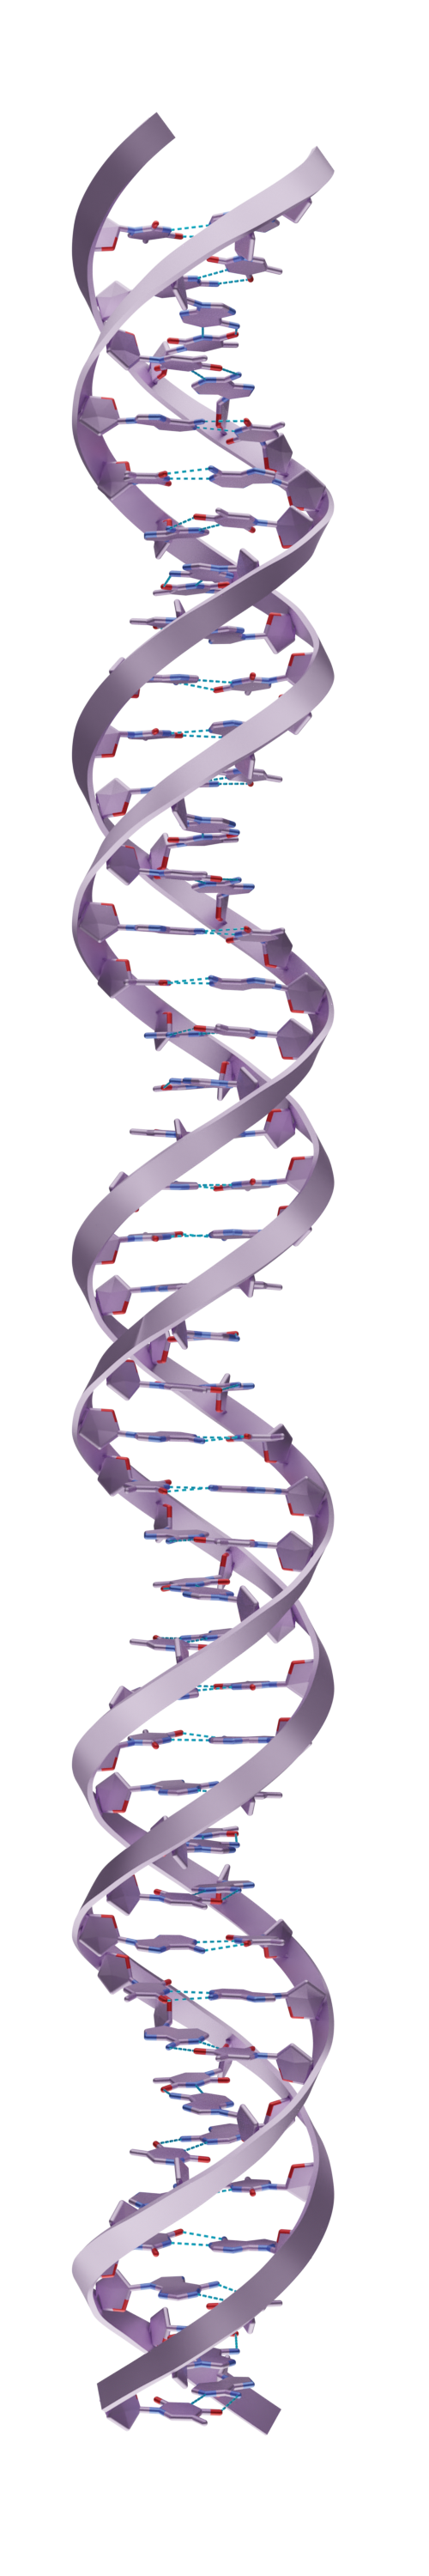
\includegraphics[width=0.20\textwidth]{Figures/DNA1.png}
  \end{center}
  \caption{caption nog maken}
\end{wrapfigure}

Deoxyribonucleic acid (DNA) is a long biopolymer composed of two strands, commonly found
in its characteristic double helical structure. DNA is most famously know for storing the
genetic code in each of our cells. The existence of this genetic code was already
postulated by the Greek philosopher Aristotle. He developed a heredity theory based
upon "blueprints" in which he tried to explain why physical traits where passed on from
generation to generation. This theory would go unnoticed until in 1869
Friedrich Meicher discovered a new microscopic substance found on discarded
surgical bandages. He would call this substance "Nuclein" since it originated
form the nucleus of the cell. Later it was found that this new substance, now called
"Deoxyribonucleic acid" or DNA, serves as a blueprints in our modern theory of
heredity.

The structure of DNA was first determined by Rosalind Franklin using X-ray
crystallography. Their research concluded that DNA consists of
two individual strands coiled around each other in a double helical structure. Each
strand is a chain of monomers, which we call nucleotides. A nucleotide is made up of a
deoxyribose sugar, phosphate group and one of four nitrogenous bases: cytosine(C),
guanine(G), adenine(A) or thymine(T). The covalent bonds that give both strands structure
are formed between consecutive phosphate groups, together they make up the backbone of
the strand. To form the double helix, two backbones are held together by
selective hydrogen bonds occurring between corresponding bases of opposing strands. These
dipole interactions give rise to a selection rule, forming only A-T and C-G pairs.

Since the binding of the two strands is mediated by hydrogen bonding, the association an
dissociation is possible. The study of these processed is called DNA thermodynamics. The
dissociation process of double stranded DNA (dsDNA) is called DNA melting, resulting in
two individual strands of single stranded DNA (ssDNA). The reverse process is called DNA
hybridisation, which is the selective binding of complementary nucleotides to form dsDNA.

The double helix structure of DNA comes in three different types, B-DNA, A-DNA and Z-DNA,
all having a slightly different geometric arrangement. In nature the B-form is most
commonly observed, it is characterised by a right-handed helix and the coplanarity
between the complementary bases as shown in Fig. ... . A helical twist of B-DNA consists
of around 10 bp's having a net helical pitch of 0.34nm. During this thesis when analysing
DNA we refer to the B-DNA form.

When Studying DNA the statistical theory polymer physics is a usefull tool. A atomistic
resolution is not needed to accuratly descibe process involving longer length scales.
Reducing the complexity of the DNA to the monomers level is often justified, allowing us
to use more general results of polymer physics.


